\chapter{Analysis}\label{analysis}
\lhead[\fancyplain{}{\bfseries\thepage}]{\fancyplain{}{\bfseries\rightmark}}

In this Chapter we explain the starting implementation and analysis of the model following biological considerations.
We will start with some numerical analysis of the model for a single cluster, and then we will analyse the evolution of an ensemble of networks made by two clusters, which hinibit each others.
The theoretical model has been analyzed making computer simulations using Python, using the well known libraries for Data Science: \emph{Numpy, Pandas} and  \emph{NetworkX}, the most famous library for network analysis. The repository is available on \href{https://github.com/riccardoscheda/thesis}{GitHub}.

\section{Single Cluster - Implementation}

For this work, we decided to create a class \emph{Random Network} to have a random boolean graph as an object, with its nodes and links, represented by a numpy array and a numpy matrix, respectively.

Every random network is a directed graph and is built to avoid self-loops, this means to create a random, boolean, and non-symmetric adjacency matrix with null trace.
\begin{figure}
\centering
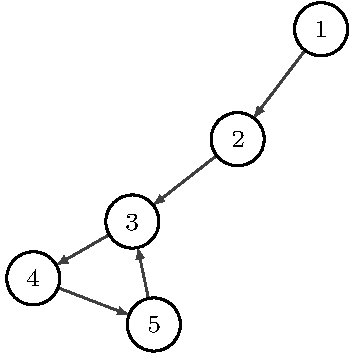
\includegraphics[scale=1]{images/singlecluster}
\caption{\emph{Example of a simple random network constructed by our Python code.}}
\label{fig:ne}
\end{figure}

For example, let's consider the network in Figure \ref{fig:ne}: the adjacency matrix $A$ of this network will be constructed as follows:
$$
A = \left (
\begin{array}{ccccc}

0 & 0 & 0 & 0 & 0  \\
1 & 0 & 0 & 0 & 0  \\
0 & 1 & 0 & 0 & 1  \\
0 & 0 & 1 & 0 & 0  \\
0 & 0 & 0 & 1 & 0  \\

\end{array}
\right )
$$
Now, we have to decide how many links per node and how many nodes have to be used for this type of network. 
As shown in Chapter \ref{model}, the discrete time evolution of the network is given by the equation:
$$
\mathnormal{\sigma_i(t+1)=\Theta\biggl(\sum_jA_{ij}\sigma_j(t)\biggr)}
$$
where $A$ is the connectivity matrix of the network.


So this means that each node which has at least one incoming link with a node which is active, in the next step this node will be active.
At each time step we can measure the average activity of the network, which is the average number of nodes with the value $\sigma_i = 1$.

\subsection{Number of links}
To choose the number of links, we considered the average activity of the network, after many iterations of the discrete evolution. In Figure \ref{fig:K} we can see that the average discrete evolution of $100$ different realizations of RBNs, with increasing size.
\begin{figure}[h]
\centering
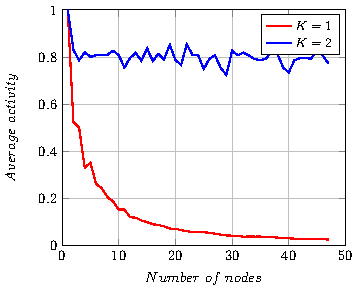
\includegraphics[scale=1.5]{images/K.pdf}
\caption{\emph{Plot of the average activity of the nodes with network of increasing size.
In the case of $K=1$ (i.e. the average number of incoming link for each network is one), the average activity decreases exponentially with the size of the network; in the case of $K=2$ instead, the average activity of the nodes remains stable with the network size.}}
\label{fig:K}
\end{figure}
In the case of $K=1$, i.e. the average number of incoming links for each network is one, the average activity decreases exponentially with the size of the network; in the case of $K=2$ instead, the average activity of the nodes remains stable with networks of increasing size. Moreover, network with only one incoming link means that the network is composed by only one big loop, which is unstable against envinromental noise. Instead, we look for networks which are stable in their state but also can be perturbed by noise. For this reason, the network considered for this model will take the parameter K constant: $K=2$.
Moreover, we can analyze the average number of outgoing links depending on the network size: In Figure \ref{fig:outgoing}, we can see that the average number of outgoing links tends to the parameter $K$.
\begin{figure}[h]
\centering
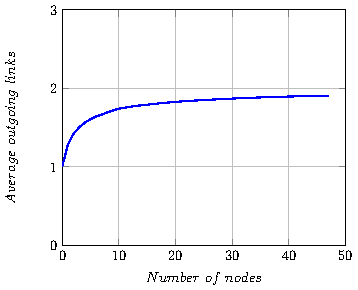
\includegraphics[scale=1.5]{images/outgoing.pdf}
\caption{\emph{Plot of the number of the outgoing links depending on the network size. We can see that the average tends to the parameter $K$. }}
\label{fig:outgoing}
\end{figure}



\subsection{Control nodes}
In simple random networks one can always find the number of independent loops.
Independent loops determine the complexity of the networks\cite{K38}, and are important for the construction of the model. In fact from the independent loops one can find the \emph{control nodes} of the network, which are the nodes that their state are able to force the state of the whole network, and are the nodes with maximum connectivity. Control nodes determine the whole activity and stability of the network. 
In RBNs with parameter $K=2$, we can see in Figure \ref{fig:loops} that the number of independent loops is linear with the network size.
\begin{figure}[h]
\centering
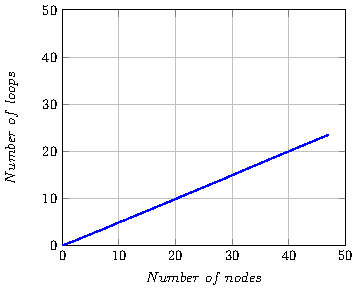
\includegraphics[scale=1.5]{images/loops.pdf}
\caption{\emph{Plot of the number of independet loops in the networks depending on the network size.}}
\label{fig:loops}
\end{figure}

Indeed, the number of control nodes grows with the number of nodes in the network, so for a big network there will be multiple control nodes. The aim is to find the right number of control nodes which are able to control the entire network activity.




\section{Noise}
The second thing to evaluate is the effect of the noise on the evolution of the network and the difference between noise and parametric noise, where parametric noise refers to the noise which infers in the links and not on the nodes.
To add noise to the system, during the discrete evolution of the network, at each time step there is a probability $p$ for the node or for the link to be turned off.
In Figure \ref{fig:noise} we can see the behavior of the average activity of the network depending on the amount of noise added. The plot is similar to a sigmoidal functions in both of the cases. In the case of noise added to the links the average activity results to be bigger than the case of noise added to the nodes. This is reasonable in the sense that since the number of links is less than the number of nodes so the effect of the noise among the links is less.
\begin{figure}[h]
\centering
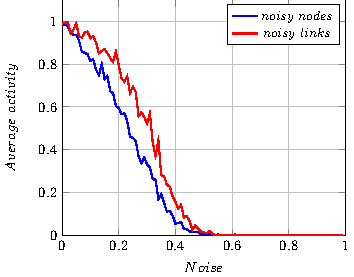
\includegraphics[scale=1.5]{images/noise.pdf}
\caption{\emph{Plot of the effect of the noise on the average activity on the network. In blue the noise works on the nodes on the network, while in red the noise works on the links. Number of nodes for each network: 10; Number of realizations for each value of noise: 100; }}
\label{fig:noise}
\end{figure}

\begin{figure}[h]
\centering
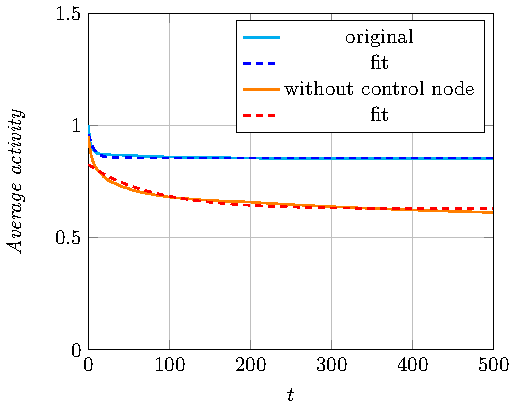
\includegraphics[scale=1.]{images/noise01.pdf}
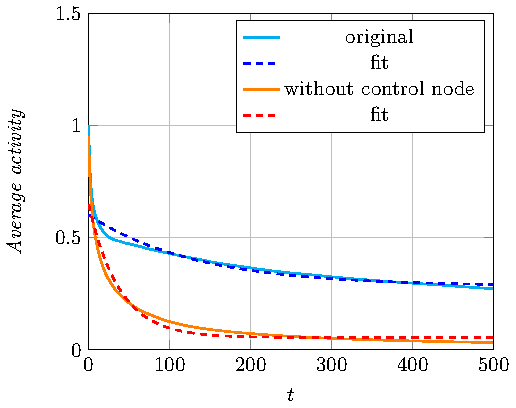
\includegraphics[scale=1.]{images/noise03.pdf}
\caption{\emph{Plot of the effect of the noise on the average activity on the network with and without control nodes. }}
\label{fig:noises}
\end{figure}

\section{Double Cluster Network}
Now we are ready to analyse the dynamics of a network composed by two different clusters. As explained in Chapter \ref{model}, two clusters will be connected by negative links with value $-1$, so we will have two clusters which hinibit the activity of the opposite cluster.
The construction of this double-cluster network is made simply by the construction of two different random networks which have each control node which connected negatively to the control node of the other cluster. In Figure \ref{fig:doublecluster} we can see an example of this type of networks.

\begin{figure}
\centering
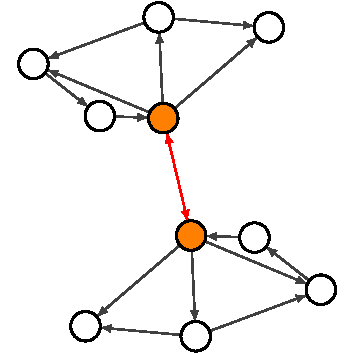
\includegraphics[scale=1.4]{images/doublecluster.pdf}
\caption{\emph{Example of double-cluster random network. Control nodes of the two clusters are connected negatively (red).}}
\label{fig:doublecluster}
\end{figure}

From double-cluster networks, what we want to find is a dynamics similar to Kramer's theory explained in Chapter \ref{kramer}. We expect to see that the activity of one cluster hinibits the activity of the other and viceversa: Adding noise to the system there will be a bistable dynamics.
The number of nodes, and the number of links of the cluster are the parameters which determine the robustness of the network. If the number of nodes of one cluster is much higher than the number of nodes of the second cluster, it will be difficult for the second cluster to hinibit the first one.
In this sense, we will have that the first cluster will remain stable even if it's disturbed by noise and by the other cluster.
